\documentclass[10pt,aspectratio=169]{beamer}
\usetheme{metropolis}
\usepackage{amsmath,amssymb}
\usepackage{booktabs}
\usepackage{graphicx}

\graphicspath{{../results/}}

\title{Orthogonal Low-Rank Transformation}
\subtitle{ECE 66200 Project 2}
\author{Weiheng Tang}
\date{\today}

\newcommand{\nuc}[1]{\left\|#1\right\|_{\ast}}
\DeclareMathOperator*{\argmin}{arg\,min}

\begin{document}
\maketitle

% --- 1 ---------------------------------------------------------------
\begin{frame}{Motivation}
\begin{itemize}
\item Many learning problems benefit from features that are
\emph{compact} per class and \emph{well separated} across classes.
\item OLT achieves both with a single nuclear-norm objective:
\[
\min_{T}\;\sum_{c=1}^{C}\nuc{TY_c}\;-\;\nuc{TY},\qquad \|T\|_2=1.
\]
\item Each $\nuc{TY_c}$ surrogates intra-class rank;
$\nuc{TY}$ subtracts the global -- gap is zero \emph{iff} class
subspaces are orthogonal.
\end{itemize}
\end{frame}

% --- 2 ---------------------------------------------------------------
\begin{frame}{Optimization: CCCP}
Difference of convex:
\[
f(T)=\underbrace{\sum_c\nuc{TY_c}}_{u(T)\text{ convex}}-\underbrace{\nuc{TY}}_{v(T)\text{ convex}}
\]
\textbf{Concave--Convex Procedure}
\begin{enumerate}
\item Linearise $-v$ around $T^{(t)}$ via subgradient
$\partial\nuc{TY}/\partial T = (UV^\top)\,Y^\top$ from SVD of $TY$.
\item Solve the convex subproblem in $T$ by a few proximal subgradient
steps.
\item Project: $T\leftarrow T/\sigma_{\max}(T)$.
\end{enumerate}
Gradient scaled by $1/N$ for dataset-size invariance.
\end{frame}

% --- 3 ---------------------------------------------------------------
\begin{frame}{Part 1.1 -- Toy: 3 non-orthogonal lines in $\mathbb{R}^3$}
\centering
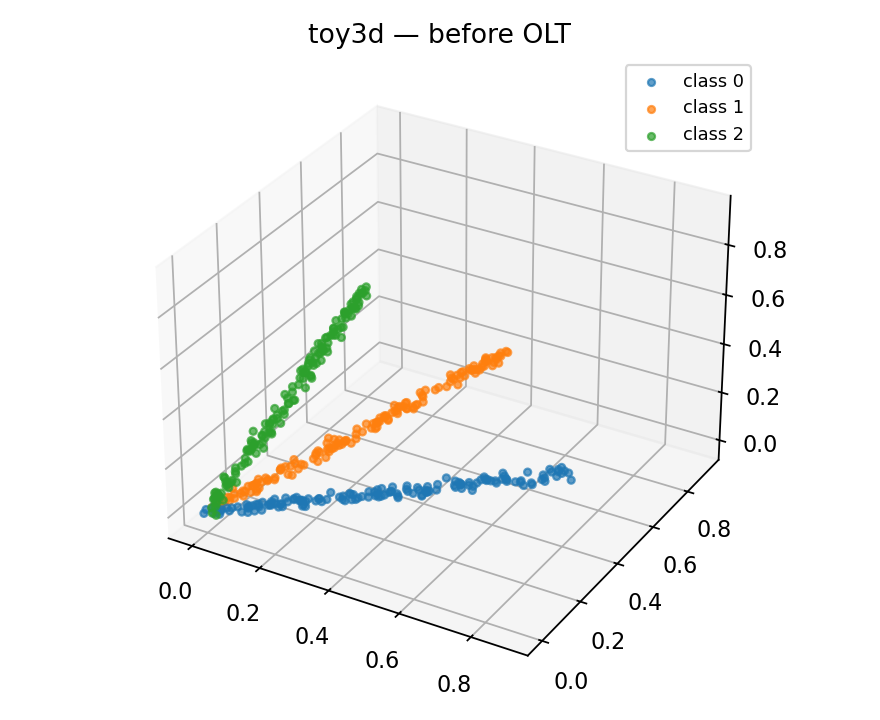
\includegraphics[width=0.32\linewidth]{part1_toy/toy3d_before.png}
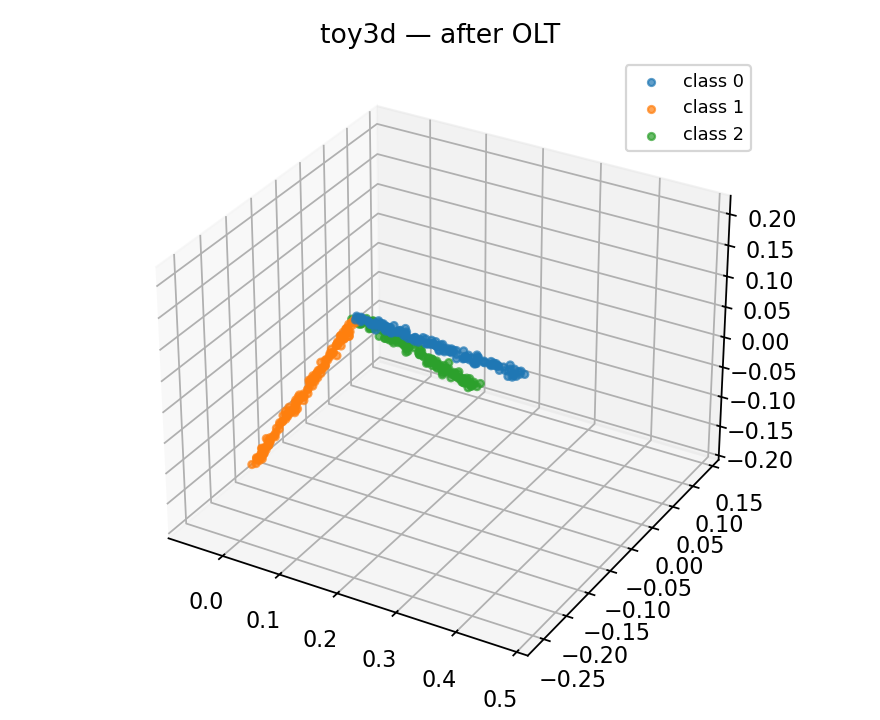
\includegraphics[width=0.32\linewidth]{part1_toy/toy3d_after.png}
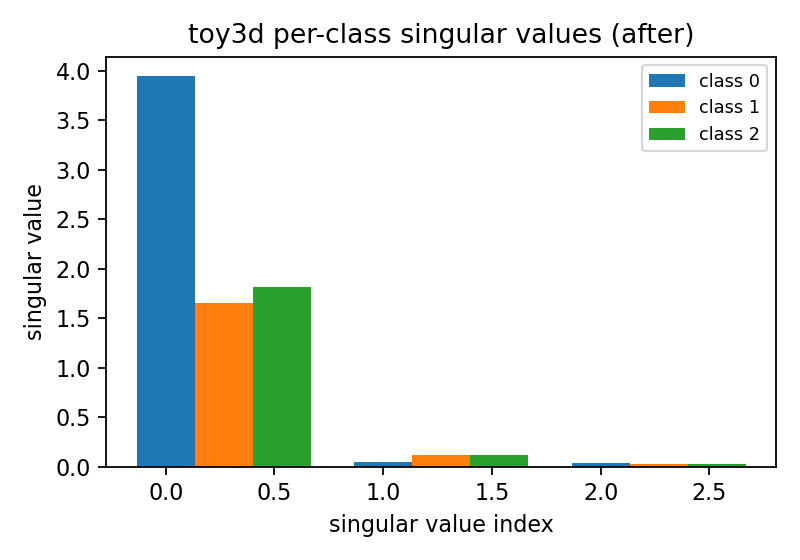
\includegraphics[width=0.32\linewidth]{part1_toy/toy3d_singvals.png}\\[0.3em]
{\small Inter-class $|\cos|$: $0.46\!-\!0.70 \;\to\; 0.01\!-\!0.14$;
per-class spectrum collapses to rank~1.}
\end{frame}

% --- 4 ---------------------------------------------------------------
\begin{frame}{Part 1.2 -- YaleB classification}
\textbf{Setup.} 38 subjects, $50/50$ split, PCA(150), $T\in\mathbb{R}^{64\times 150}$,
60 CCCP iters. Inference: \emph{nearest subspace}
$\hat c=\argmin_c\|(I-B_cB_c^\top)Tx\|$.

\vspace{0.5em}
\centering\small
\begin{tabular}{lc}
\toprule
\textbf{Method} & \textbf{Test acc} \\\midrule
PCA + nearest subspace & $0.843$ \\
LDA & $0.910$ \\
\textbf{OLT + nearest subspace} & $\mathbf{0.949}$ \\
\bottomrule
\end{tabular}
\hfill
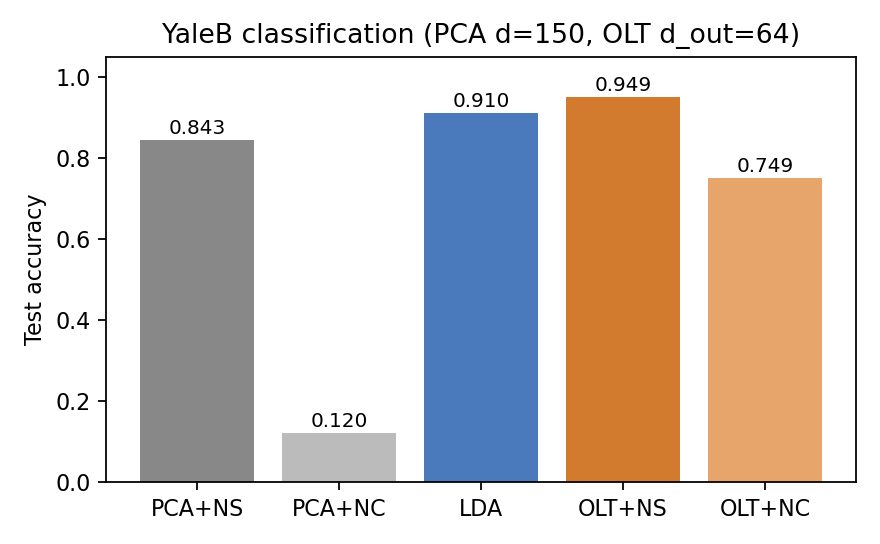
\includegraphics[width=0.42\linewidth]{part1_yaleb/yaleb_accuracy.png}
\end{frame}

% --- 5 ---------------------------------------------------------------
\begin{frame}{Part 1.3 -- Subspace clustering on YaleB}
\textbf{Pipeline.}
$k$NN graph $\to$ spectral pseudo-labels $\to$ OLT supervised by
pseudo-labels $\to$ \emph{nearest-subspace reassignment in OLT space}
(``cluster$\to$classify via OLT'').

\vspace{0.5em}
\centering\small
\begin{tabular}{lccc}
\toprule
& Acc & NMI & ARI \\\midrule
$k$NN + spectral & $0.229$ & $0.279$ & $0.055$ \\
\textbf{OLT + NS} & $\mathbf{0.350}$ & $\mathbf{0.435}$ & $\mathbf{0.186}$ \\
\bottomrule
\end{tabular}
\hfill
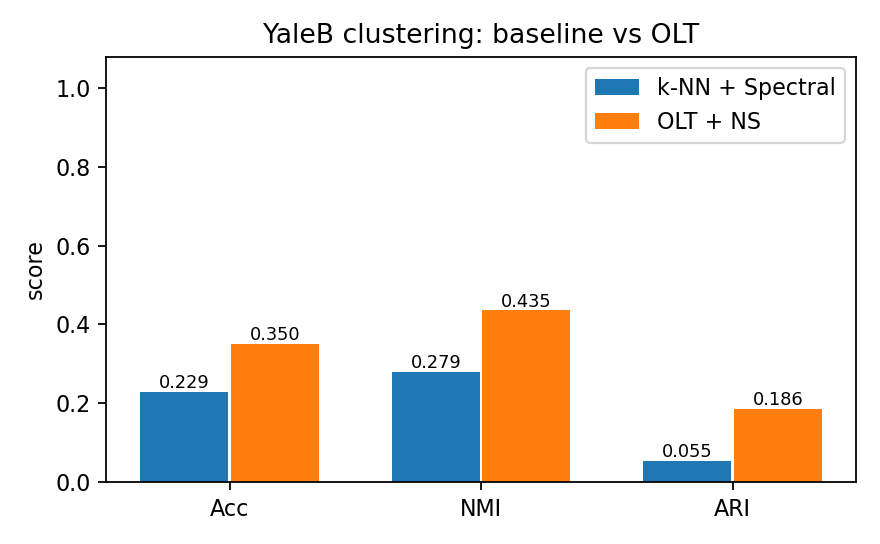
\includegraphics[width=0.42\linewidth]{part1_yaleb/yaleb_clustering.png}
\end{frame}

% --- 6 ---------------------------------------------------------------
\begin{frame}{Part 2.1/2.2 -- Modality-invariant OLT on MNIST}
\textbf{Modalities.} Original MNIST + Rotated MNIST ($\pm 45^\circ$),
PCA(50), $d_{\text{out}}=20$.

\textbf{Joint formulation.}
$Y_c^{\text{joint}}=[Y_c^o,Y_c^r]$ -- forces both modalities into the
\emph{same} per-class subspace.

\vspace{0.5em}
\centering\small
\begin{tabular}{lcc}
\toprule
Transform & $\to$ orig & $\to$ rot \\\midrule
$T_o$ & $0.698$ & $0.475$ \\
$T_r$ & $0.559$ & $0.516$ \\
$\mathbf{T_{\text{joint}}}$ & $\mathbf{0.745}$ & $\mathbf{0.636}$ \\
\bottomrule
\end{tabular}
\hfill
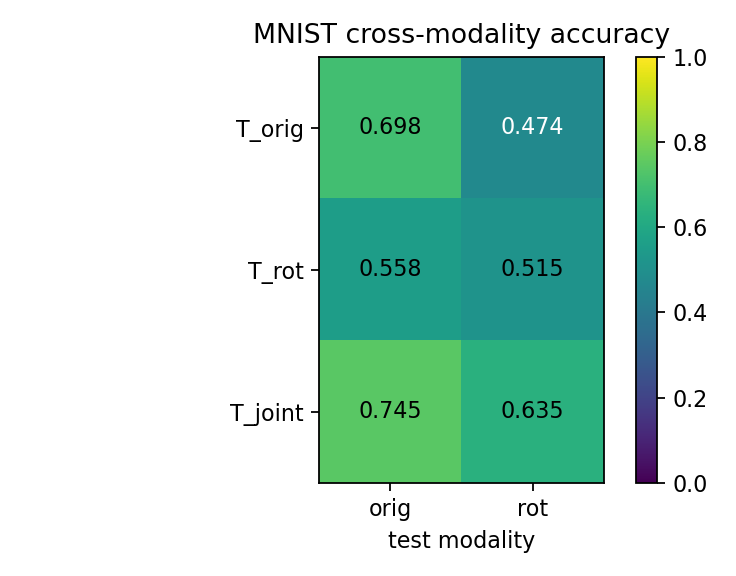
\includegraphics[width=0.40\linewidth]{part2/mnist_cross_modality.png}
\end{frame}

% --- 7 ---------------------------------------------------------------
\begin{frame}{Part 2.3 -- Joint OLT on frozen CNN features}
Train pytorch/examples MNIST CNN, freeze, extract 128-d features,
fit joint OLT on $[F^o,F^r]$.

\vspace{0.6em}
\centering\small
\begin{tabular}{lcc}
\toprule
& Orig & Rot \\\midrule
Frozen CNN head (fc2)    & $0.9924$ & $0.8639$ \\
CNN feat + NS (no OLT)   & $0.9896$ & $\mathbf{0.8989}$ \\
CNN feat + OLT + NS      & $0.9850$ & $0.8811$ \\
\bottomrule
\end{tabular}
\hfill
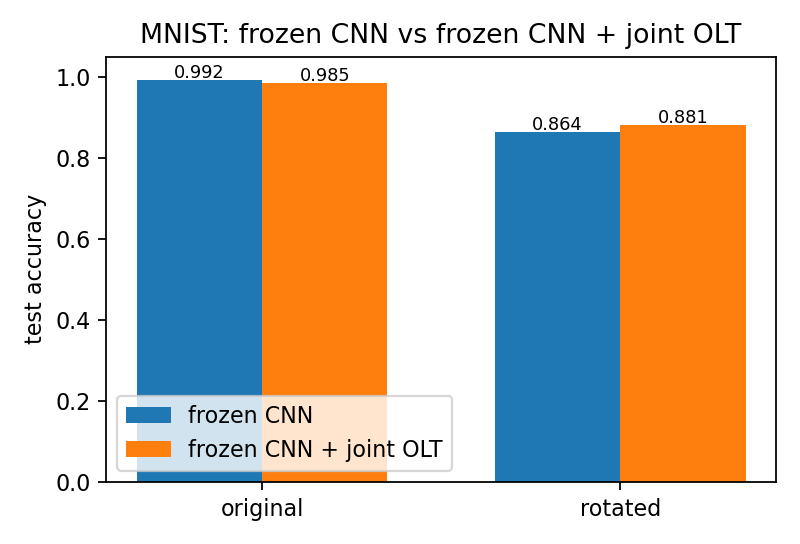
\includegraphics[width=0.42\linewidth]{part2/mnist_frozen_vs_olt.png}\\[0.4em]
{\small In this experiment, OLT \emph{hurts} ($-1.8$ on rotated vs.\ the
fair NS baseline). The nuclear-norm linear prior mismatches the
nonlinear, ReLU-activated CNN features.}
\end{frame}

% --- 8 ---------------------------------------------------------------
\begin{frame}{Part 3 (Option A) -- OLT as a CNN regularizer}
Insert the same nuclear-norm functional as a differentiable batch loss:
\[
\mathcal{L}=\mathrm{CE}(W f_\theta(x),y)\;+\;\lambda\,
\frac{1}{|\mathcal{B}|}\!\left(\sum_c\nuc{F_c}-\nuc{F}\right)
\]
\begin{itemize}
\item Geometric prior on \emph{the whole class subspace}, not only its mean.
\item Differentiable through PyTorch's SVD.
\item No supervision other than mini-batch labels.
\end{itemize}
\end{frame}

% --- 9 ---------------------------------------------------------------
\begin{frame}{Part 3 -- Results (10 epochs, identical seed)}
\centering\small
\begin{tabular}{ccccc}
\toprule
$\lambda$ & Orig & Rot & $\nuc{F}/\sum_c\nuc{F_c}$ & note \\\midrule
$0.0$ & $0.9919$ & $0.8582$ & $0.577$ & baseline \\
$\mathbf{0.1}$ & $\mathbf{0.9921}$ & $\mathbf{0.8653}$ & $0.812$ & \textbf{best} \\
$0.5$ & $0.9914$ & $0.8598$ & $0.947$ & saturated \\
$1.0$ & $0.7926$ & $0.6195$ & $0.971$ & collapse \\
\bottomrule
\end{tabular}\\[0.6em]
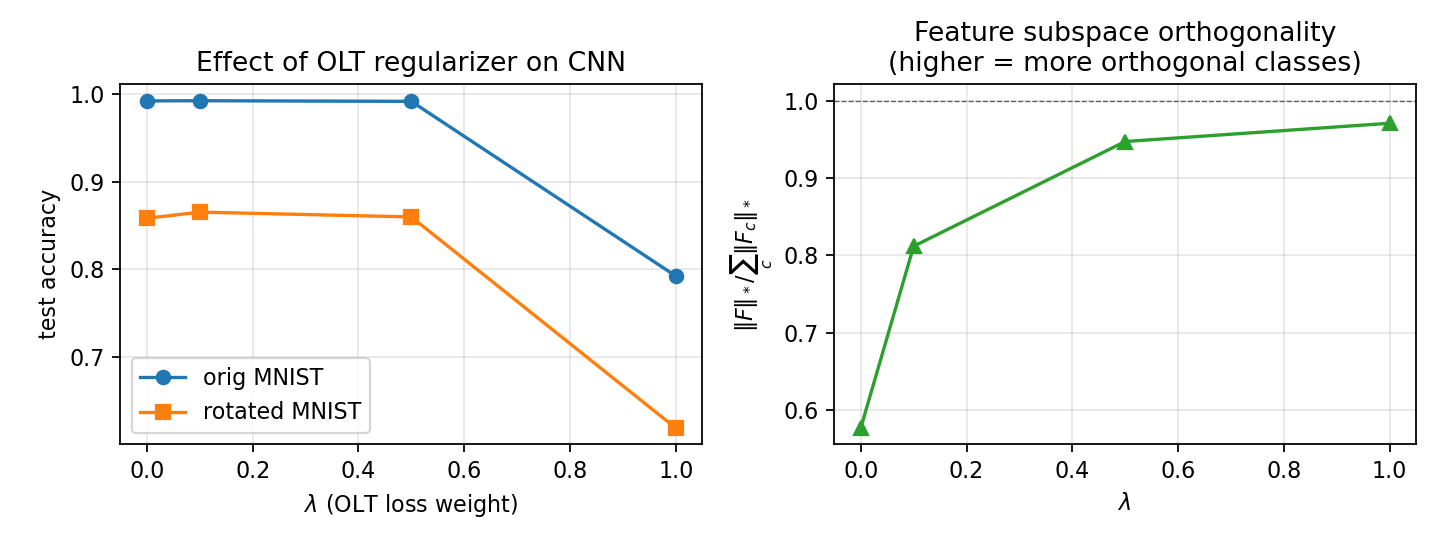
\includegraphics[width=0.85\linewidth]{part3/part3_lambda_sweep.png}
\end{frame}

% --- 10 --------------------------------------------------------------
\begin{frame}{Take-aways}
\begin{itemize}
\item One nuclear-norm functional jointly enforces \emph{intra-class
low rank} and \emph{inter-class orthogonality}.
\item CCCP solver is short ($<\!200$ lines) and works across faces
and digits.
\item Empirical wins:
\begin{itemize}
\item YaleB classification: \textbf{$+4$ pts over LDA}.
\item YaleB clustering (38-way): \textbf{$\sim\!3.4\!\times$ ARI lift}.
\item Cross-modality MNIST: \textbf{$+16$ pts} on rotated test.
\item OLT-regularized CNN: matches CE on clean, \textbf{$+0.7$} on rotated,
with measurable orthogonality of the learned feature space.
\end{itemize}
\item Limitations: post-hoc OLT hurts on frozen CNN features
(linear prior vs.\ nonlinear ReLU); SVDs per batch (modest cost);
very large $\lambda$ overpowers cross-entropy.
\end{itemize}
\end{frame}

\end{document}
